\documentclass[../main.tex]{subfiles}

\begin{document}

\section{Approach overwiew}
\label{section:lauxus:approach}

\begin{figure}[h]
    \centering
    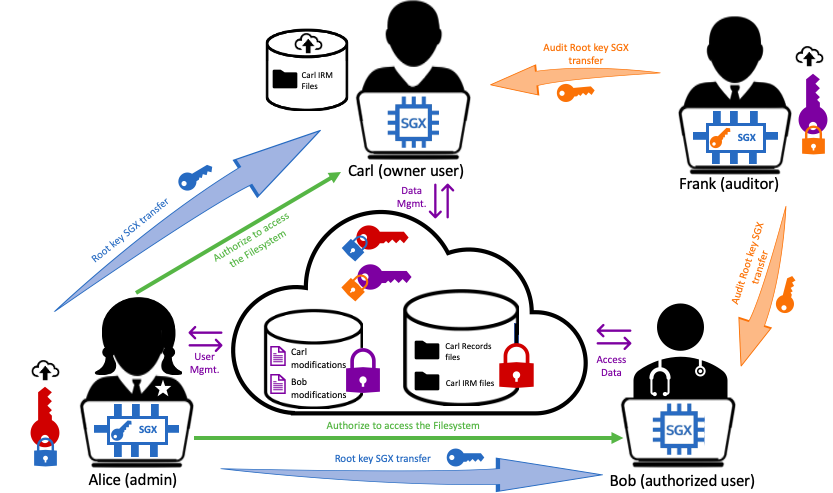
\includegraphics[width=\textwidth]{../../images/lauxus/approach}
    
    \caption{Overview of the protocol to share the FileSystem}
    \label{figure:lauxus:approach}
\end{figure}

\par After all the previous introduction sections, we can start to explain the solution we designed to address the problem. In this section, we will explain the solution at a high level. The Figure \ref{figure:lauxus:approach} presents this protocol and will be the heart of this section. Detailed insights will be discussed in the Chapter \ref{chapter:lauxus}.
\par As presented in the use case Section \ref{section:problem:use_case} the protocol happens between multiple parties. By comparing with the Figure \ref{figure:problem:use_case}, we see that we have one more actor here: the administrator (Alice). We didn't talked about her in the previous section as it was not necessary for understanding the goals and the general idea of the problem. The role of the administrator is to create the filesystem and upload it to the cloud storage. She is also responsible for the user management: registering and assigning specific roles to each user.

\par Next, we will take a look at the core of the filesystem, its content. In order to protect confidential information against attacker, the administrator will encrypt the filesystem with a secret key (the root key, in red). Then she will upload the encrypted filesystem to the remote storage. In order to avoid sharing the root key in clear, she will only share it after encrypting it with another key (the blue key). This last key will only be transmitted to authorised users through a secure out-of-band channel. This is where all the power of SGX comes into action: being able to manipulate a secret on a client's computer without revealing any information on this secret to the client itself. Here, the secret we are talking about is the root key. In this way, the intended user, for example Carl, can decrypt the key located on the storage and retrieve the root key. Then he is able to access and decrypt the filesystem. This means that every party must have an SGX-enabled CPU on their computer. The blue key, once shared, will be securely stored on each computer by leveraging SGX sealing capabilities.

\par Last, we have the auditing files. There is a 1-to-1 mapping between the auditing files and the files in the filesystem. In practice, the filesystem will create one entry in the appropriate audit file on each read or write of any user, no matter its role. We are using two different keys in order to have segregation of duties (the administrator manages \textbf{only} the filesystem and the auditor manages \textbf{only} the audits). The idea being that an organisation, here the hospital, can't at the same time read in plaintext the filesystem content and the auditing files. We don't want an organisation to change the auditing file at their advantage. As audit files are used for GDPR purposes, only a trusted entity should read those, thus owning the audit root key. They work in a similar manner than the filesystem content. The equivalent of the administrator is the auditor who owns an audit root key (the purple key). The sharing of the audit root key follows the exact same procedure as with the root key. As explained above, the audit root key must also be securely shared in order to have a working filesystem.

\par An UML state diagram can be found in Appendix \ref{appendix:state_diagram} for more detailed information. % change / important ?


\end{document} 